\chapter{State of the art}
This chapter will go through relevant articles and already known knowledge on the subject of mixed criticality systems. It will also explain the EMC2DP.

\section{Mixed criticality systems}
%SotA regarding MCS.
A MCS is achieved by letting applications of different criticality share resources. These resources could be computational power in the CPU, memory, peripherals, input/output ports. As of July 2016, the most explored area is sharing the CPU between multiple criticality levels \cite{burns2016}. \\

Potential benefits with pursuing MCS as opposed to distributed systems are reduced physical space required, reduced weight, reduced heat generation, reduced power consumption and reduced production costs~\cite{burns2016}. % Potential downsides are increased complexity which would lead to higher system design costs.

\subsection{Economical benefits of MCS}
%Lower production cost, higher design cost?

\subsection{Sharing processor}
Vestal, Burns.

%Schedulers
1. (audsley) 2. EDF-VDL

For a more complete review of work done on MCSs with a shared processor, see the paper by~\cite{burns2016}.

\subsection{Different criticality on different processors}


\subsection{Sharing memory}
%http://pertsserver.cs.uiuc.edu/~mcaccamo/papers/euromicro12.pdf

\section{Current system}
\label{sec:lit_emc2mcs}
%Describe current system more in depth.
The EMC2DP uses two operating systems, a RTOS for safety-critical applications and a GPOS for non-critical applications. A Virtual Machine Monitor (VMM) or "Hypervisor" is used to alternate between safety-critical RTOS and non-critical GPOS. The RTOS is TOPPERS FMP kernel \cite{website:FMP}, and the GPOS is a custom modified Linux distribution. The VMM used is SafeG \cite{website:safeg}. It switches processor state via a hardware switch. See figure~\ref{fig:modeswitch}.

\begin{figure}[H]
\centering
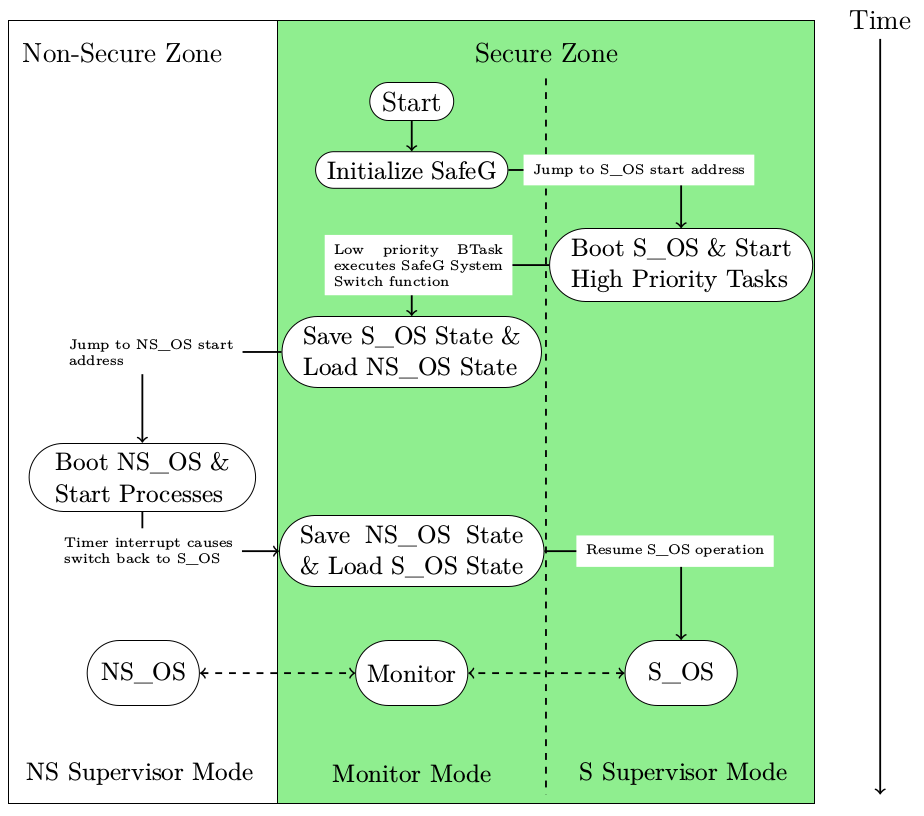
\includegraphics[width=\textwidth]{./img/literature_modeswitch.png}
%Flowchart of how the physical CPU switches between the virtual CPUs
\caption{Flowchart of the boot sequence of the CPU. \cite{zaki2016}}\label{fig:modeswitch}
\end{figure}

A Field Programmable Gate Array (FPGA) as interface between processor and board. Peripherals are separated as secure and non-secure using ARM TrustZone \cite{website:ARM}, see section~\ref{sec:trustzone}. \\ %TODO: Expand!

An overview of the system can be seen in Figure~\ref{fig:introduction_overview}.

\begin{figure}[H]
\centering
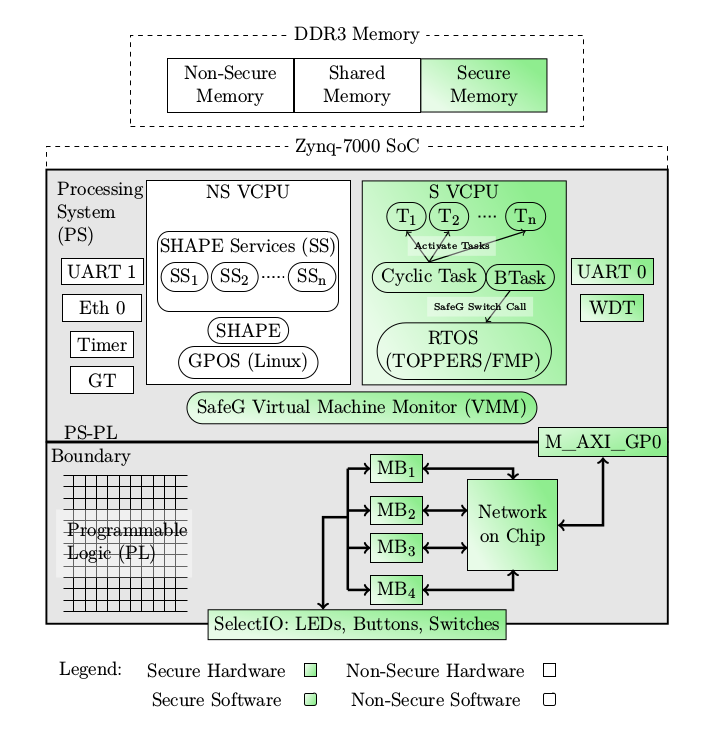
\includegraphics[width=\textwidth]{./img/introduction_overview.png}
\caption{System overview of the MCS in place.\cite{zaki2016}}\label{fig:introduction_overview}
\end{figure}

%Linux:
%Root File System
%Device Tree
%Kernel

%Boot SD:
%uboot

%FMP:
%compiled RTOS

\subsection{TrustZone}
\label{sec:trustzone}
"TrustZone is a security extension available in modern ARM processors that creates a security infrastructure designers can use to protect critical system assets. This infrastructure is achieved by enabling the partition of system components, both hardware and software, into either a Secure and a Normal world (or zone). Resources that are marked as normal are not permitted to access Secure zone components. This mechanism is enforced by the AMBA3 (Advanced Microcontroller Bus Architecture) AXI (Advanced eXtensible Interface) bus system. It contains an extra control signal for each of the read and write channels (Non-secure or NS bits) that dictate the access rights Non-secure bus masters to the Secure slaves. Each processor with an enabled TrustZone security extension can be partitioned into a Normal and a Secure virtual CPU. The virtual processors execute in a time-multiplexed fashion, and use the ”Monitor Mode” state to create an efficiently switching mechanism between Normal and Secure zones. The NS-bit, bit[0] of the Secure Configuration Register (SCR) in the System Control Coprocessor (CP15), controls the activation of secure state of the processor. Whenever the NS-bit set high, the processor state immediately switches to the Normal world. However, if the processor is in Monitor Mode, it remains in the Secure world regardless of the state of the SCR NS-bit. The processor state can nter monitor mode by either issuing a special instruction, SMC (Secure Monitor Call), in software or by hardware exception mechanisms such as IRQ, FIQ, external Data Abort, or external Prefetch Abort. In general, the software running in monitor mode serves the purpose of saving the state of the current world, and loading the state the other."~\cite{website:ARM} \\ %TODO: Wording

\section{Standards}

\subsection{AUTOSAR}

\subsection{ASIL}

\begin{table}[h]
\begin{tabular}{|c|c|c|c|c|}
\hline
\multirow{2}{*}{Severity class} &\multirow{2}{*}{Probability} &\multicolumn{3}{|c|}{Controllability class} \\ \cline{3-5}
& &C1 &C2 &C3 \\ \hline
\multirow{4}{*}{S1} & E1 & QM & QM & QM \\ \cline{2-5}
 & E2 & QM & QM & QM \\ \cline{2-5}
 & E3 & QM & QM & A \\ \cline{2-5}
 & E4 & QM & A & B \\ \hline
\multirow{4}{*}{S2} & E1 & QM & QM & QM \\ \cline{2-5}
 & E2 & QM & QM & A \\ \cline{2-5}
 & E3 & QM & A & B \\ \cline{2-5}
 & E4 & A & B & C \\ \hline
\multirow{4}{*}{S3} & E1 & QM & QM & A \\ \cline{2-5}
 & E2 & QM & A & B \\ \cline{2-5}
 & E3 & A & B & C \\ \cline{2-5}
 & E4 & B & C & D \\
\hline
\end{tabular}
\caption{ASILs as a function of severity, probability and controllability.}
\label{table:ASIL}
\end{table}